\chapter{The Local Atomic Environment}
\label{chap:invariance}
\section{Introduction}
Vol.~35 of Solid State Physics is dedicated to electronic structure
theory from the point of view of the local environment. This perspective
has a long tradition in physical and chemical electronic structure theory.
This chapter is purely a summary of the work developed there.

Given a Hamiltonian Haydock's Recursion method gives a rapidly convergent 
scheme for computing quantities of interest. The primary quantity of interest 
is the density of states. When this has been computed comparisons between the energetics of 
structures can be made. The method is applicable in situations where Bloch's theorem no longer holds.
A situation which arises at surfaces, in glasses, disordered structures, in structures with a substantial
quantity of impurites, vacancies, defects and dislocations. In short the method is applicable
in realistic physical situations and yields quantities which can be interpreted directly.

%Topics that are often discussed at the beginning of introductory physics courses include:
%the study of black body radiation, photoemission phenomenon, De Broghlie waves,
%electron diffraction experiments and the structure of the hydrogen atom.
%Examination of these topics constitute a suitable foundation 
%for understanding the formalism and experimental justification for the theory.

%It is natural to hope that from the understanding of the electronic states of hydrogen the
%understanding of larger atomic systems, containing progressively more electrons, might emerge. 
%However as the number of electrons in a system grows the wave function becomes 
%somewhat unwieldly to work with and the accurate evaluation of the 
%electron-electron repulsions becomes more difficult. Computers provide a route
%to numerical solutions of the equations governing the behaviour of these systems.
%Computer simulations are commonly performed these days in many branches of physics, 
%chemistry, engineering, and biology. The use of computers to solve Schr\"odinger's 
%equation for electrons in crystals has led to the proliferation of the 
%many, many tribes of electronic structure theory. 
%The tribes are well known to practitioners in the field. A non-exhaustive list
%of some of these we can name here as: tight binding and linear combination of atomic orbitals (LCAO), 
%linear muffing tin orbitals (LMTO), plane waves and pseudopotentials, Gaussian orbitals, and 
%Kohn-Kuttinger-Rostiger theory.
%While successful in a number of respects numerical work can be tedious and, more importantly, can obscure underlying
%mechanisms. There is also a tendency for people working in numerical methods to become 
%excessively obsessed with algorithmic details and, most importantly,
%the results of a single calculation may not provide a framework that accounts for a range
%of phenomenon in homologous series of materials where only slight adjustment of the physical
%interaction parameters change. (This speaks to Ehrenreich third observation 
%that results for homologous materials should be computed
%wherever possible and the results should be compared). 

An example of the economy of explanatory expression afforded by the recursion method
and a physical formulation in terms of the local atomic environment
is Ref.~\cite{johannes76}. In that work 76 crystal structures are correctly predicted 
with a model containing 5 coefficients derived from first principles.

The purpose of this chapter is two fold: firstly to attempt to summarize the incredible range and
detail of theory and application covered in Vol. 35 of Solid State Physics. The secondly
purpose is to speculate on where it should be possible to exploit modern 
computational advantages and the new understanding which has emerged in materials 
to systematically improve descriptions of quantum systems based
on the local environment. 

%

\section{The Invariance Theorem}
\label{sec:invariance}
Heine presents an extended discussion of the invariance
theorem. Heine's section begins, by way of introduction, by pointing 
out an analogy between the the local density of states of a system of interacting
electrons and the black body spectrum of electromagnetic radiation.
Weyl [1911 Math. Ann. 71 441] demonstrated demonstrated the total density
of modes is independent of the shape of the cavity so long as the
radiation is contained in a cavity with dimensions greater than the wavelengths
under consideration. Von Laue [1914 Ann. Phys. Lpz 44 1197] demonstrated that the local density of modes at 
a particular point are exponentially insensitive to the cavity walls.

This analogy has been developed by Friedel [1954 Adv. Phys. 3 446] where
the substition is electromagnetic modes for electronic wavefunctions and
the probability density for finding an electron at a given point
with a given energy replaces the local density of normal modes.\cite{annett94}

The analogy can be seen by writing the density of states,
and the local density of states (for each spin direction) as:
%
\begin{eqnarray}
n(E) = \sum_{n}\delta(E-E_{n}) \\
n(E,\r) = \sum_{n} |\psi_{n}(\r)|^{2}\delta(E-E_{n})
\end{eqnarray}
%
The local density modes of black-body radiation alternatively can be written:
%
\begin{equation}
\rho(\omega,\r)= \sum_{i} |\bra \r| \psi_{i}\ket|^{2}\delta(\omega-\omega_{i}),
\end{equation}
%
with $\psi_{i}$ the eigenfunction (of an electromagnetic wave or a wavefunction) for an eigenvalue $\omega_{i}$.\cite{annett94}
The normal modes of a system can be quite quite sensitive to disturbances but the 
local density of modes, averaged over a small frequency interval, is a stable quantity 
insensitive to disturbances more than a few wavelengths away.

The local density of states is related in turn to the diagonal elements of
the Green's function of a system:
%
\begin{equation}
n(E,\r) = -\frac{1}{\pi}{\rm Im}~G(\r,\r,E)
\end{equation}
%

\section{Matching Green's Functions}
The following treatment has been developed by Heine which in turn follows the 
work of Garcia-Moliner and Rubio, and, Velicky and Bartos, Refs.~\cite{garcia69, velicky71, garcia71},
along with the work of Inglesfield in Refs.~\cite{inglesfield71,inglesfield81}.

An intuitive grasp of the theory of matching Green's functions is a key component of a material
modellers outlook. The theme will be returned to time and again throughout these notes and in
practical applications. Entire subfields of materials science which at first appear distinct 
are in effect just different methods of solving the Schr\"odinger equations in a convenient
basis for one region and matching it at the boundary to a convenient basis 
for a solution in another region. Embedding one potential in another, treating impurities,
the interaction between valence electrons and core electrons bound tight to the nucleus all
involve in one way or another matching Green's functions across a surface.

%The perspective that Heine introduces in Vol. 35 of Solid State Physics 

First a change of variables is perform from $\r$ to $\r''$ in 4.1 
and $\r$ to $\r''$ and $\r'$ to $\r$ in 4.3:
%
\begin{equation}
\label{eq:greentot}
[-\frac{1}{2}\nabla^{2}_{\r''} + V(\r'') - E]G(\r'',\r',E)= -\delta(\r''-\r')
\end{equation}
%
\begin{equation}
\label{eq:greenA}
[-\frac{1}{2}\nabla^{2}_{\r''} + V(\r'') - E]G_{A}(\r,\r'',E)= -\delta(\r''-\r')
\end{equation}

Now multiply Eq.~\ref{eq:greentot} by $G_{A}$ and Eq.
\ref{eq:greenA} by $G$ Then integrate over $\r''$ over region A using
Green's theorem:
%
\begin{equation}
\label{eq:greenthm}
\int\int\int(\phi\nabla^{2}\psi - \psi\nabla^{2}\phi)d^{3}\r 
= \int(\phi\nabla\psi-\psi\nabla\phi)d{\mathbf{S}}
\end{equation}
%
We suppress the energy arguments from here on in assuming them to be contained in G. 

obtained by expressions for $G$ by integrating $\r''$ over region $A$.
%
\begin{equation}
\label{eq:green1a}
G(\r,\r') = G_{A}(\r,\r') + \frac{1}{2} \int d\mathbf{S} 
[\frac{\partial G_{A}(\r,\r_{s})}{\partial n_{S}}G(\r_{S},\r') - G_{A}(\r,\r_{S})\frac{\partial G(\r_{S},\r')}{\partial n_{S}}] [\r, \r' \in A]
\end{equation}

$\frac{\partial}{\partial n_{S}}$ denotes the normal component of grad across
the surface S and $\r_{S}$ is a point on S. (The grad term is a directional component
so the sign can change depending on the orientation.)

And in region B:
%
\begin{equation}
\label{eq:green1b}
G(\r,\r') = G_{B}(\r,\r') - \frac{1}{2} \int d\mathbf{S} 
[\frac{\partial G_{B}(\r,\r_{s})}{\partial n_{S}}G(\r_{S},\r')
- G_{B}(\r,\r_{S})\frac{\partial G(\r_{S},\r')}{\partial n_{S}}] [\r, \r' \in B]
\end{equation}
%

A further property has been used:
%
\begin{equation}
G(\r,\r',E) = G(\r',\r,E),
\end{equation}
%
which is often justified on the ground of a time reversal theorem applying 
to the wave functions in the system.

Finally consideration of the case where $\r'$ and $\r''$ are in different regions is required.

With $\r''$ in B and $\r'$ in A Eq.~\ref{eq:greentot} becomes:
%
\begin{equation}
[-\frac{1}{2}\nabla^{2}_{\r''} + V(\r'') - E]G(\r'',\r') = 0,
\end{equation}
%
the delta function is uniformally zero with those spatial constraints.

The next case restricts $\r$ in B:
%
\begin{equation}
[-\frac{1}{2}\nabla^{2}_{\r''} + V(\r'') - E]G_B(\r,\r'')= \delta(\r-\r''),
\end{equation}
%

A similar cross multiplying trick gives:
%
\begin{equation}
\label{eq:green1c}
G(\r,\r') = -\frac{1}{2} \int dS[\frac{\partial G_{B}(\r, \r_{S}}{\partial n_{S}} G(\r_{S},\r')
- G_{B}(\r, \r_{S})\frac{\partial G(\r_{S},\r')}{\partial n_{S}}] \quad [\r~{\rm in}~B, \r'~{\rm in}~A],
\end{equation}
%
and a similar relation for [$\r$ in A and $\r'$ in B].

Eq.~\ref{green1a} and Eq.~\ref{green1b} give solutions for G but 
aren't very useful until the terms $G(\r_S,\r)$ and 
$\frac{\partial G}{\partial n_{S}}$ are eliminated.

From Eq.~\ref{eq:green1a} we let $\r$ tend to the boundary so $\r = \r_{S}$
%
\begin{equation}
\label{eq:greensys1}
G(\r'',\r') = G_{A}(\r''_{S}, \r') + \frac{1}{2} \int d{S}
[\frac{\partial G_{A}(\r''_{S}, \r_{S})}{\partial n_{S}} G(\r_{S},\r) - 
G_{A}(\r''_{S},\r_{S})\frac{\partial{G(\r_{S}, \r')}}{\partial n_{S}}].
\end{equation}
%

The second relation comes from Eq.\ref{eq:green1c} with 
$\r$ in region B and letting $\r$ tend to $\r^{''}_{S}$.
%
\begin{equation}
\label{eq:greensys2}
G(\r''_{S}, \r') = -\frac{1}{2}\int dS [\frac{\partial G_{B}(\r''_{S}, \r_{S})}{\partial n_{S}}
-G_{B}(\r''_{S},\r_{S})\frac{\partial G(\r_{S},\r')}{\partial n_{S}}]
\end{equation}
%

We now dump the cumbersome indices on the position attributes. These
were necessary to motivate the physical argument for how we have a Green's function
description in one region of space, a Green's function description in another, 
and the joined physical system should be some combination of these two descriptions
which match at the interface. The final step is to write Eq.~\ref{eq:greensys1} 
and Eq.~\ref{eq:greensys2} as matrices:
%
\begin{align}
\label{eq:operator1}
g = g_{A} + \frac{1}{2}\G'_{A}g - \frac{1}{2}\G_{A}g' \\
g = -\frac{1}{2}\G'_{B}g + \frac{1}{2}\G_{B}g' \\
\end{align}
%
\begin{align}
\label{eq:operator2}
g & = & [\G^{-1}_{A}(1-\frac{1}{2}\G'_{A}) + \G^{-1}_{B}(1+\frac{1}{2}\G'_{B})]^{-1} \G^{-1}_{A}g_{A} \\
g' & = & [(1-\frac{1}{2}\G'_{A})^{-1}\G_{A} + (1+\frac{1}{2}\G'_{B})^{-1}]^{-1}(1 - \frac{1}{2}\G'_{A})^{-1}2g_{A}
\end{align}
%
$g$, $g_{A}$, $g'$ are vectors in a space $\{\r_{S}\}$ with components $G(\r_{S},\r')$,
$G_{A}(\r_{S},\r')$, $\partial G(\r_{S},\r')/\partial n_{S}$ with $\r'$ fixed.

$\G_{A}$, $\G'_{A}$ are operators in the space with matrix elements
$G_(A)(\r''_{S}, \r_{S})$, $\partial G_{A}(\r''_{S}, \r_{S})/\partial n_{S}$.

Where the inverse in Eq.~\ref{eq:operator1, eq:operator2} 
doesn't exist there is a pole. This is the condition for a discrete energy level 
of the Schrodinger equation for the combined A + B systems. 

Equations written in the form of \ref{eq:green1a} are of the type required for the invariance theorem namely:
%
\begin{equation}
G(\r,\r';E) = G_{A}(\r,\r';E) + {\rm boundary ~ corrections},
\end{equation}
%
where we have restored the energy argument.
These considerations provide a reasonable mathematical framework for 
investigating electronic structure from the point of view of the local environment.
Indeed as Heine himself says: 

\begin{quote}
The importance of this approach would lie in the fact that
one has a single entity $G_{A}$ to represent an element in anything 
from a small molecule to a complex alloy.
\end{quote}

As a practical example the success of planewave and pseudopotential methods 
is reliant on finding decent approximations to the quantity $G_{A}$. The plane waves
in the interstitial regions must match the Green's function for the atomic system
at a particular radial cutoff and energy. If a function can be found that 
describes the scattering of these waves across a suitable energy range the approximation 
is a good one and the matching of the two systems will be successful. This
is represented schematically in Fig.~\ref{fig:pseudosplit}.
%
\begin{figure}
\begin{center}
\includegraphics{./invariance/pseudosplit.png}
\caption{Schematic representation of decomposing the Green's function into a local atom centered
Green's function, $G_{A}$, and the Green's function in the interstitial region $G_{B}$.
A pseudopotential is a function that allows $G_{B}$ to be represented as a relatively
smooth function of position capable of efficient description in terms of plane waves.
The functions must match at the cutoff for $G_{A}$ to the solutions for 
atomic wave functions. Another approach would involve matching the $G_{A}$ 
and $G_{B}$ explicitly at each stage of the calculation until self-consistency is obtained.}
\end{center}
\end{figure}
%
Heine's ambition turns on this:
%
\begin{quote}
We see now that the trick in the new formulation of quantum 
mechanics is not just to express measurable quantities in terms of 
G, {\it but in terms of some appropriate small parts of G that can be solved 
for and computed separately from all the unwanted remainder of G.}
\end{quote}
%
This relies, again in analogy with black bodies, on the Green's
function in a certain region of space being independent of the size and shape
of the container and the boundary conditions.

\section{Slater-Koster Tight Binding}
  Let us denote the translation operator $\hat{T}$
as the operator which displaces all the coordinates of a vector 
by a crystal lattice vector $\R_{i}$ we require 
firstly that $[\hat{T},\hat{H}]=0$, i.e. that the 
translation operator commutes with the Hamiltonian. This also
has the consequence that the eigenvectors of the Hamiltonian
must be eigenvectors of the translation operator. 

Bloch's theorem encapsulates this idea. When a translation operator acts 
on a Bloch state of a crystal the wavefunction is multiplied by a scalar
value $e^{i\k\cdot\R}$: i.e. the condition for a vector to be an
eigenvector.

If a basis set of atomic orbitals $\phi_{n}(\r-\R_{i})$
is placed on each atom in the crystal an un-normalized Bloch sum can be 
written as $\sum_{\R_{i}} e^{i\k\cdot\R_{i}}\phi_{n}(\r-\R_{i})$. For
a given $\k$ there will be off-diagonal elements between Bloch sums
for different atomic orbitals.


The matrix elements between Bloch sums (where L\"owdin orbitals $\psi_{n}$ 
are used instead of LCAOs, \cite{lowdin62}) gives:
%
\begin{equation}
\sum_{\R_{j}} e^{i\k\cdot(\R_{j}-\R_{i})}\times\int \psi^{*}_{n}(\r-\R_{i})H\psi_{m}(\r-\R_{j})dV
\end{equation}
%
The development of computers means the secular equations can be solved 
at arbitrary $\k$ points. \footnote{The paper explicitly anticipates that the integrals and Bloch 
sums could be performed with the help of computers: ``The possibility is not excluded 
that eventually ways will be found to do this work by means of high-speed computers, but
it will certainly be quite out of the question without such help."} 

The work of Slater-Koster demonstrates, in an intuitive fashion, how localized atomic
states, when modulated by a wave of the form $e^{i\k\cdot\R}$ can interfere 
(constructively or deconstructively) to allow charge to accumulate in different 
spatial patterns between atoms, and how the variation in the eigenvalues of $H_{\k}$
can give rise to band structures. Determining the coefficients involved in the 
tight binding energy integrals is somewhat involved. The Coordinate system needs
to be set up and the integrals performed for different combinations of spherical
harmonics on neighbouring atoms. Ref.~\cite{sharma79,podolsky04} both give explicit
expression for generating the coefficients programmatically.

The determination of the integration constants is a problem unto itself.
Tight binding parameters for the transition metals can be extracted from 
a number of places: tight binding parameters that span the transition
metal range can be found in Refs. \cite{nieminen76}, \cite{pettifor77} and \cite{jepsen75, andersen77, harrison80}.
Harrison has also published a set of universal parameters for s-p bonded structures.

\section{Transition Metal Tight Binding}
\label{sec:tmtb}
Bullet discusses some of the problems with treating d electrons in a tight binding 
formalism (Sec. IV 13 Solid State Physics Vol. 35). Fig.~\ref{fig:datoms} demonstrates
one of the main issues arising with d electrons:
%
\begin{figure}
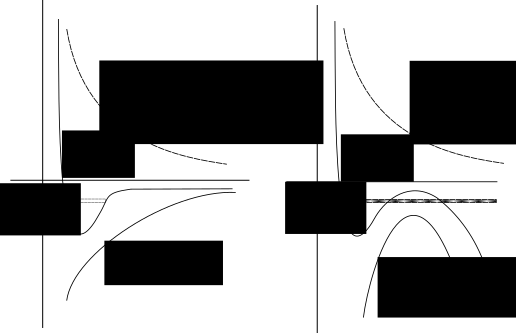
\includegraphics{./invariance/resonant-datoms.pdf}
\caption{The possibility of free electron states, in the interstitial region, 
resonating with atom centered localized states. The centrifugal components of the 
atomic d wave scattering channel can combine with
the atomic potential to produce a bound electronic state at some energy $E^{0}_{l}$ for an atomic system.
In a crystal the atomic periodic potential can be such that electrons can be bound in an
atomic d-like state can have the same energy as tunnel through the barrier localizing 
them and mix with free electron plane wave states. This dual character of the wave 
function, with localized components and extended components, requires careful 
detangling to return to a tight binding description. This difficulty 
stems from the presence of an energy resonance 
complicating the process of choosing the coefficients of the tight binding matrix. 
For the optimal, energy independent, set of coefficients that can be 
chosen see the work of Pettifor. There is a close parallel with the resonant
scattering of d-wave electrons in materials and Feshbach resonances Ref.~\cite{chin10}.
[Figure Taken from D.W. Bullet Solid State Physics Vol. 35 pg. 197.]}
\end{figure}
%

From pseudopotentials we are familiar with having to match the logarithmic energy
derivative at some cutoff radius. Usually found by integrating the radial
Schr\"odinger equation to find $u_{l}(r,\epsilon)$ and matching the logarithmic derivatives:
%
\begin{equation}
L_{l}(\epsilon) \equiv \frac{u'_{l}(r_{0},\epsilon)}{u_{l}(r_{0},\epsilon)} = \frac{\kappa[j'_{l}
(\kappa r_{0}) - \tan \eta_{l} n'_{l}(\kappa r_{0})]} {j_{l}(\kappa r_{0}) - \tan \eta_{l} n_{l}'(\kappa r_{0})]},
\end{equation}
%
where
%
\begin{equation}
\label{eq:phaseshift}
\tan \eta_{l} = \frac{\kappa j'_{l} - L_{l}j_{l}}{\kappa n'_{l} - L_{l}n_{l}}.
\end{equation}

In terms of the energy and width the l=2 phase shift Eq.~\ref{eq:phaseshift} 
can be written:
%
\begin{equation}
\label{eq:dshift}
\tan \eta_{d} = \frac{\frac{1}{2}W(\epsilon)}{\epsilon_{d}-\epsilon}.
\end{equation}
%
The uncertainty principle allows for the estimation of the rest
time for an electron on an atomic d state to be around $\hbar/W_{d}\approx 10^{-14}$s \cite{friedel73}.
\footnote{Ref.~\cite{friedel73}, written in 1973, provides us with another example
of the early impact electronic computers were making in the field. Friedel  compares 
the relative merits of `muffin tin' type calculations and tight binding approximations.
The former approach he describes as leading, ``to fairly exact if cumbersome
computations, and has thus had the support of the `computers lobby'". The conclusion
puts forward a number of points in favour of tight binding approaches as 
being suitable for studying complex phases and lattice defects,
latent heats of phase changes, elastic constants and electron-phonon couplings.}

The strong centrifugal contribution to the
atomic scattering potential from higher angular moment channels means the effective potential
can create a bound atomic state. In a solid the energy of this bound state can match the 
energy of a free electron state in the interstitial region and there will
be resonant tunneling between the two states. This results in the hybridization of d states
and plane waves. 

This means an appropriate model Hamiltonian must account for the various states as
%
\begin{eqnarray}
\label{eq:d-hamiltonian}
H =  d-d  &  d-PW \\
     PW-D & PW-PW 
\end{eqnarray}
%
where d-d and PW-PW are of the tight-binding and plane-wave 
pseudopotential form and hybridization occurring in the 
off-diagonal elements. The dual characteristic of transition metals
tightly bound d-electrons and diffuse s-p orbitals hybridizing 
accounts for the difficulties in describing their electronic properties.


The $dd\sigma$ terms behave roughly as \cite{pettifor71}:
%
\begin{equation}
\label{eq:pettifor}
dd\sigma \approx \frac{-5W\cos\kappa_{d}R}{\kappa_{d}R}
\end{equation}
%
If we write our basis functions in terms of localized orbitals
Eq.~\ref{eq:pettifor} suggests our Hamiltonian matrix will be 
populated by a huge number of off-diagonal matrix elements which can't be neglected. If 
the energy is equal to $k^{2}$ constructive interference occurs and the energy summation
diverges with off-diagonal matrix elements between all d states on remote atoms becoming
significant. This isn't entirely surprising. We are considering a periodic crystalline solid
and the eigenfunctions of this crystal are extended throughout. The off-diagonal elements
in a coordinate space representation reflect the long range order of the material and
preservation of the phase of the electronic wave function as they move from atom to atom. See
Chapter~\ref{chap:odlro} for further discussion of this and related points.

The `best' approximations to the explicit formulas for $dd\sigma$, $dd\pi$ and $dd\delta$ and the phase
shift $d_{0}'$ of the diagonal tight-binding elements 
These difficulty have been addressed in a number of works 
\cite{hubbard67}, \cite{hubbard68}, \cite{hubbard69} \footnote{Another computational
snapshot comes from Ref.~\cite{hubbard69}, "...smaller secular 
equations are used, taking about one second per k point on an IBM  360/65." The
main storage capacity of those machines was 524 kilobytes. See Fig.~\ref{fig:ibm360}
for a (grainy) snapshot of what that computer looked like.},
and J. Hubbard, ibid 2, 1222 (1969). The problem being to define an
energy independent Hamiltonian, amenable to tight binding for the d electrons.

Deriving an effective, tight binding, energy indepedent parameterization
of d electron structure  culminated in the work of D. G. Pettifor's \cite{pettifor69}. 
Pettifor's work produced a justifiable scheme for computing the two center tight binding integrals of Slater
and Koster, $dd\sigma$, $dd\pi$, $dd\delta$ in terms of the position and halfwidth of the resonance:
$\epsilon_0$ and $\Gamma$. It is worthwhile considering the achievement of these collected papers.
With relatively limited computing power the workers determined 
the positions of atomic eigenvalues, band widths, and the effect 
of atomic scattering potentials. In 
the course of the work a great deal of algebraic manipulation of spherical 
harmonics and plane waves is required, along with the determination
of numerical values via graphical methods. All in all a laborious but fruitful task resulting
in energy independent matrix elements localized to nearest (next nearest ) 
neighbours real and reciprocal space.

The work of Pettifor and colleagues in determining justifiable tight 
binding parameters for transitional metals, 
effectively completed by 1969, was an important prerequisite for the subsequent 
development of the recursion method in the 1970s. Generalized tables for tightbinding parameters 
across the transition metal series has been produced in Ref.~\cite{harrison80}.

%The parameters used in Ref.~\cite{burke78} are appropriate to the BCC structure.
%The tightbinding Hamiltonian only considers two center contributions, with the parameters 
%coming from Pettifor\cite{pettifor69} and rescaled to produce the observed
%bandwidth of tungsten. The parameters are given in Table~\ref{tab:dsurface}.

For ease of reference we collect here d tight-binding coefficicents
that have found there way into the literature. The choice of these parameters
is very much an example of theoretical materials science constituting a 
craft. In later chapters we will examine some of the developments that set
tight-binding and the choice of coefficients on a more definite 
theoretical framework. The Slater-Koster parameters used for FCC, BCC, 
and HCP crystals in Ref.~\cite{haydock72} are given in Table \ref{tab:pettiparams}.
%
\begin{table}
\begin{center}
\begin{tabular}{|c|c|c|c|c|} 
\hline
Structure & $dd\sigma$ & $dd\pi$  & $dd\delta$ &  Band-limits \\
\hline
FCC       & -0.027784  & 0.012535 & -0.001554  & -0.131 to 0.085 \\ 
\hline
HCP       & -0.027784  & 0.012535 & -0.001554  & -0.119 to 0.081 \\
\hline
BCC       & -0.03248   & 0.01538  & -0.00200   & -0.119 to 0.097 \\
          & -0.01341   & 0.00487  & -0.00049   &              \\
\hline
\end{tabular}
\caption{Slater-Koster parameters from Pettifor \cite{pettifor69}, 
along with band edges in Ry. First and second nearest neighbour 
parameters are given for BCC crystals. \label{tab:pettiparams}.}
\end{center}
\end{table}
%
%\begin{table}
%\begin{tabular}{|c|c|c|}
%\hline
%SK Parameter & First Neighbour & Second Nearest Neighbour \\
%\hline
%$dd\sigma$ & -0.02992  & -0.05364 \\
%$dd\pi$    &  0.06652  &  0.01943 \\
%$dd\delta$ &  0.00800  &  0.00196 \\
%\hline
%\end{tabular}
%\caption{These parameters are difficult to make out from the electronic version of Ref.
%due to poor resolution of the scan. \label{tab:dsurface}.}
%\end{table}
%
\begin{table}
\begin{center}
\begin{tabular}{|c|c|c|}
\hline
\multicolumn{3}{|c|} {FCC TB Parameters} \\
\hline
Integral & 1st Nearest Neighbour & 2nd Nearest Neighbours \\
\hline
$dd\sigma$ & -0.027784 & - \\
$dd\pi$    &  0.012535 & - \\
$dd\delta$ & -0.001554 & - \\
\hline
\multicolumn{3}{|c|} {BCC TB Parameters} \\
\hline
Integral & 1st Nearest Neighbour & 2nd Nearest Neighbours \\
$dd\sigma$ & -0.06560  & -0.03195 \\
$dd\pi$    &  0.04373  & 0.02130\\
$dd\delta$ & -0.010934 & -0.00537\\
\hline
\end{tabular}
\caption{The tight binding parameters used for the example recursion 
calculations in this chapter, in the FCC lattice only nearest neighbours 
are included.}
\end{center}
\end{table}

Whether we are able to create a tight binding description of transition metals
depends on whether a decent, energy independent, approximation to the electronic 
structure in fcc/bcc metals can be achieved with 9x9 matrices describing 
nearest neighbour interactions of the s, p and d states, in the Slater-Koster 
form or derived from electronic states localized according to some 

\subsection{Kelly Tight Binding}

An example from Kelly helps to make the application of the tightbinding scheme clear:
%
\begin{quote}
As input data we require a convenient local representation of $H$. In simple crystals,
this is most easily given in terms of interactions with a unit cell and between neighboring cells.
For a FCC transition metal we have nine orbitals (1 s-orbital, 3 p-orbitals, and 5 d-orbitals) per site, 
and a diagonal 9x9 matrix for the self-energies of these orbitals. Twelve 9x9 matrices 
suffice to describe the interaction of any atom with its nearest neighbours.
\end{quote}
%

The actual operation of $H|u_{n}\ket$,which has been discussed in a general way so far, 
can be written as:
%
\begin{equation}
H|u_{n}\ket = \sum_{\alpha l \beta j}a_{n \alpha l}(\bra \beta j |H| \alpha l\ket)|\beta j\ket,
\end{equation}
%
to exploit the sparsity of H we introduce an index $z$ which runs over the neighbors of 
site l with which the orbitals interact:
\begin{equation}
H|u_{n}\ket = \sum_{\alpha l z}a_{n \alpha l}(\bra \beta_{z} j_{z} |H^{z}|\alpha l\ket)|\beta_{z} j_{z}\ket.
\end{equation}
There are no restrictions on the number of orbitals per site, or on the range of interactions that can be
incorporated, these only impact on the efficiency of the method and the validity of the original assumptions
about the dominance of the local atomic environment.


\section{Recursion Method}
The principle of the recursion method is to obtain a convergent expression 
for an element of the Green's function:
%
\begin{equation}
G_{\chi\chi}(E) = \bra\chi|[E + i\delta -H]^{-1}|\chi\ket.
\end{equation}
%

The Green's function can be immediately related to the local density of states as:
%
\begin{equation}
n_{\alpha l}(E) = -\frac{1}{\pi} {\rm Im}\bra\alpha l|[E + i\delta -H]^{-1}|\alpha l\ket
\end{equation}
%

The state $\chi$ which we project on to can be made up of some linear combination 
of the local basis set $\phi_{\alpha l}$, which, in turn, could be local atom centered orbitals, bond orbitals, 
Wannier functions, atomic diplacements, or any localized quantity we wish to define. The method is thus
applicable to a wide range of problems in condensed matter. In short what we wish to examine
is determined by the choice of $\chi$.

\subsection{Mathematical Origin}
The trick of the recursion method, if you like to think of things in terms of tricks, 
or its generating feature, if you prefer, is that from the outset the `Greenian', the element
of the Green's function we are interested in, is restricted to a particular matrix element: 
%
\begin{equation}
\label{eq:greenian}
G_{00}(E) = \bra u_{0}|[E-H]^{-1}|u_{0}\ket 
\end{equation}
%
As Heine puts it in his chapter:
%
\begin{quote}
Note that we do not want the whole of the inverse matrix $[E-H]^{-1}$, 
\emph{only one element}, and on this the whole method depends. In physics we do not
usually inquire about the whole of life, but about one particular matrix element (at a time) and we have chosen
$u_{0}$ so that Eq.~\ref{eq:greenian} gives us what, to put it crudely, we want.
\end{quote}

If we are given a tridiagonal matrix of the form:
%
\begin{equation}
H = \begin{bmatrix}
a_0 & b_1 & 0 & 0 & 0 &  ...\\
b_1 & a_1 & b_2 & 0 & 0 &  ...\\
0 & b_2 & a_2 & b_3 & 0 &  ...\\
0 & 0 & b_3 & a_3 & b_4 & ...\\
0 & 0 & 0 & b_4 & a_4 & ...  \\
0 & 0 & 0 & 0 & b_5 & ... 
\end{bmatrix}
\end{equation}

%
The determinants and sub-determinants etc. of the matrix can be nested:
%
$$
\newcommand*{\temp}{\multicolumn{1}{|c|}{b_1}}
\newcommand*{\tempa}{\multicolumn{1}{|c|}{b_2}}
\newcommand*{\tempb}{\multicolumn{1}{|c|}{b_3}}
\newcommand*{\tempc}{\multicolumn{1}{|c}{0}}
\begin{array}{|ccccccc}
\cline{0-5}
a_0 & b_1 & 0 & 0 & 0 & 0  & D_0 \\ \cline{2-6} 
\temp & a_1 & b_2 & 0 & 0 & 0 & D_1 \\ \cline{3-6} 
0 & \tempa & a_2 & b_3 & 0 & 0 & D_2 \\ \cline{4-6}
0 & \tempc &  \tempb &  a_3 & b_4 & ... & D_3
\end{array}
$$

Eq.~\ref{eq:greenian} can be rewritten in terms of its determinants:
%
\begin{equation}
\label{eq:greendet}
\bra u_{0}|[E-H]^{-1}|u_{0}\ket = \frac{{\rm det}|D_{1}|}{{\rm det}|D_{0}|},
\end{equation}
%
or, equivalently, be written as:
%
\begin{equation}
\label{eq:greendet}
\bra u_{0}|[E-H]^{-1}|u_{0}\ket = \frac{1}{\frac{{\rm det}|D_{0}|}{{\rm det}|D_{1}|}}.
\end{equation}
%
Appeal is then made to Cauchy\footnote{Baron Augustin-Louis Cauchy FRS FRSE (21 August 1789 – 23 May 1857)} 
for the following expansion:
%
\begin{equation}
\label{eq:cauchy}
{\rm det}|D_{0}| = (E-a_{0}){\rm det}|D_{1}|-b^{2}_{1}{\rm det}|D_{2}|
\end{equation}
%
and when generalized to determinants for $|D_{n}|$, $|D_{n+1}|$, and $|D_{n+2}|$:
%
\begin{equation}
\frac{{\rm det}|D_{n}|}{{\rm det}|D_{n+1}|} = E-a_{n}-\frac{b^{2}_{n+1}}{\frac{{\rm det}|D_{n+1}|}{{\rm det}|D_{n+2}|}}
\end{equation}

\footnote{
%C. Lanczos J. Res. Natl. Bur. Stand. 45, 255 (1950) 
%used the chain model in numerical work as a way of diagonalizing matrices
%that could be implemented efficiently in a computer.
Chebyshev used chain models for approximating functions on an interval
P. L. Chebyshev, Bull. Acad. Imp. Sci. St. Petersbourg 1, 193 (1859)}

%\begin{equation}
%b_{n+1}|u_{n+1}\ket = H |u_{n}\ket - a_{n}|u_{n}\ket - b_{n}|u_{n-1}\ket
%\end{equation}

\section{Analytic Recursion}
\subsection{The Constant Chain}
The simplest chain model that can be handled analytically is the constant chain and it
serves as the paradigm of all the recursion calculations that will be undertaken. 
The constant chain corresponds to the general continued fraction written:
%
\begin{equation}
\label{eq:constantchain}
G_{0}(E) = \cfrac{1}{E-a_{0}-\cfrac{b_{1}^2}{E-a_{1}-\cfrac{b_{2}^{2}}{E-a_{2}-\cfrac{b_{3}^{2}}{...}}}},
\end{equation}
%
where $a_{0}=a_{1}=...=a_{n}$ and $b_{0}=b_{1}=...=b_{n}$. 
%
In this chain an electron experiences the same pull to 
every site on the chain, and can hop from one site to 
the next with the same hopping amplitude $b^{2}_{n}$. 
%
That all the coefficients are the same means a closed 
form solution can easily be found by recognizing that 
Eq.~\ref{eq:constantchain} can be written as:
%
\begin{equation}
G_{0}(E) = \frac{1}{E-a-b^{2}G_{0}(E)},
\end{equation}
%
and rearranged to give:
%
\begin{equation}
G_{0}(E) = (\frac{E-a}{2b^{2}}) \pm \sqrt{\frac{1}{4}(\frac{E-a}{b^{2}})^{2} - \frac{1}{b^{2}}}.
\end{equation}

The argument of the Green's function is $E + i\delta$, for positive 
energies the negative root is chosen and for negative energies 
the positive root is chosen. This gives the real
and imaginary part of the Green's function plotted 
in Fig.~\ref{fig:gfconstchain}.
%
\begin{figure}
\begin{center}
{\graphicspath{{./invariance/chain_figs/}}\input{./invariance/chain_figs/chain_plot.tex}}
\caption{Real and imaginary parts of the Green's function for the constant chain.\label{fig:gfconstchain}}
\end{center}
\end{figure}
%
The constant chain yields an analytic solution. All the coefficients of the continued
fraction are known and the recursion relation can be solved exactly. In practice
the computation of the $a_{n}$ and $b_{n}$ terms is truncated after some number.
The function chosen to approximate the remaining coefficients is discussed in
Refs.~\cite{haydock84, haydock85}.

A great deal of interesting physics can be obtained directly from the chain model. 
For instance, to couple an impurity to a constant chain we allow the first two coefficients $a_{0}$ and $b_{1}$ to vary, 
and the rest of the chain remains constant. This leads to the expression:
%
\begin{equation}
\label{eq:defectchain}
G(E) = \frac{1/b_{1}}{\frac{E-a_{0}}{b_{1}} - G_{0}(E)}
\end{equation}
%
There are a few different cases depending on the relative magnitude of $a_0$ 
and $b_{1}$ and the chain parameters $a$ and $b$.
We plot the behaviour of the function for a few different choices of coupling parameters
$b_{1}$, and the relative position of the defect state $a_0$ in Fig.\ref{fig:gfdefect}. 
We will return to the idea of coupling single particle states to bands in Chap.~\ref{chap:manybodyrec}. 

In Fig.~\ref{fig:inband} the defect state energy is placed inside the energy range of the band. The
results for different couplings $b_{1}$ are plotted.
%
\begin{figure}
\begin{center}
{\graphicspath{{./invariance/chain_figs/}}\input{./invariance/chain_figs/inband_plot.tex}}
\caption{Defect chain model, Eq.~\ref{eq:defectchain}, with $a_{0}$ chosen to be 
within the band of energies for the constant chain. The strength of the coupling between the chain 
and the defect, $b_1$, is varied. For well matched systems the density of states splits 
into two resonances corresponding to bound and antibound states. \label{fig:impurity}}
\end{center}
\end{figure}
%

For $a_{0}$ outside the energy range of the band, the coupling to the band shifts the position
of the pole from $a_{0}$ and adjusts the areas under the two curves. Where there is 
near matching of the chain and the defect the function changes rapidly for small
variations in the coupling parameters.
%
\begin{figure}
\begin{center}
{\graphicspath{{./invariance/chain_figs/}}\input{./invariance/chain_figs/adsorbate_plot.tex}}
\caption{Coupling of an adsorbate to a constant chain model Eq.~\ref{eq:defectchain}. 
In this case $a_{0}$ is chosen to be outside the band formed by the chain.
Where there is strong coupling to the chain two distinct resonances appear.
The blue and green curves correspond to couplings of $b_{1}=2b$ and $b_{1}=b/10$ respectively.
\label{fig:gfconstchain}}
\end{center}
\end{figure}
%
In cases where the defect state is far removed and only weakly coupled to the band
there is only a small renormalization of the pole from $a_{0}$ and redistribution of the weight across the band.
This will be discussed more in Chap.\ref{chap:manybodyrec} in the context of single particle states
interacting with plasmon bands and the continuum.

\section{The Cambridge Recursion Library: \texttt {CamRecLib}}
Moving from analytic chain models to material systems with different atoms requires specification
of the Hamiltonian. The choice of the tight binding parameters was discussed in the first half of this
chapter. For present purposes the Slater-Koster tight binding parameters for the interaction of 
d-electrons should be sufficient to demonstrate the important features of typical recursion type calculation.
In subsequent chapters we will prefer the use of tight binding parameters based on Wannier functions.

\subsection{Integrals of the Density of States}
%
As will be seen, and is perhaps already known to the reader, nothing is perfect. The
recursion method for all its many strengths has an issue: the chain must be terminated
somewhere. In an extended system only so many moments can be computed in practice.  
This is not necessarily a defect of the method but a reflection of reality. Though
this is disappointing there is a silver lining. Integrals over the density of states
are very stable. As such any time we require an integral over the density of states
we can be quite confident in the result, similarly integrals over differences
are quite stable. This property of the recursion chains will be exploited again and again
to compute the relative stability of different structures. The details of how
integrals of continued fractions are performed is included in the appendix 
but it is highly recommended that the reader refer to Ref.~\cite{nex78}
for a formal description of the implemented techniques.

To compute the difference in energy between inequivalent structures 
one begins with the electron occupancy of a specific orbital:
%
\begin{equation}
N_{\alpha l}(E) = \int_{-\infty}^{E_{F}} n_{\alpha l}(E') dE'
\end{equation}
%

The total energy in a particular orbital:
%
\begin{equation}
U_{d} = \int_{-\infty}^{E_{F}}E'n_{\alpha l}(E') dE'
\end{equation}
%

The energy difference of two structures A and B can also be computed
to high accuracy:
%
\begin{eqnarray}
\label{eq:Ua}
U_{A} = \int_{-\infty}^{E_{FA}} E n_{A}(E) dE
\end{eqnarray}
%
\begin{eqnarray}
\label{eq:Ub}
U_{B} = \int_{-\infty}^{E_{FB}} E n_{B}(E) dE
\end{eqnarray}
%
\begin{equation}
\label{eq:totaldos}
Z = \int_{-\infty}^{E_{FA}} n_{A}(E)dE = \int_{-\infty}^{E_{FB}}n_{B}(E)dE
\end{equation}
%
\begin{equation}
U_{A}-ZE_{FA}= \int_{-\infty}^{E_{FA}}(E-E_{FA})n_{A}(E)dE
\end{equation}
%
\begin{equation}
U_{B}-ZE_{FA}= \int_{-\infty}^{E_{FA}}(E-E_{FA})n_{B}(E)dE + \int_{E_{FB}}^{E_{FA}}n_{B}(E)dE
\end{equation}
%
If $n_{B}(E)$ is taken to be constant across that small energy range, the second term, in
Eq. results in a small squared term that can be dropped. Swapping $E_{FB}$ and $E_{FA}$ gives
a similar result. This justifies dropping the A index on the Fermi energy to get the
final expression \cite{johannes76}:
%
\begin{equation}
U_{A}-U_{B} = \int_{-\infty}^{E_{F}}(E-E_{F})[n_{A}(E) -n_{B}(E)]dE.
\end{equation}
%

\subsection{Local Density of States}
\label{sec:fccldos}
The simplest demonstration of the Cambridge Recursion Library 
is a computation of the local density of states for an Ni atom located at the center of a small cluster. 
Fig.~\ref{fig:cuboid} depicts a 75 atom cuboid cluster and the computed local density of states for an 
Ni atom located in the middle of the cluster. 
The contribution of the electronic states to the total energy are also plotted. 
%
\begin{figure}
\begin{center}
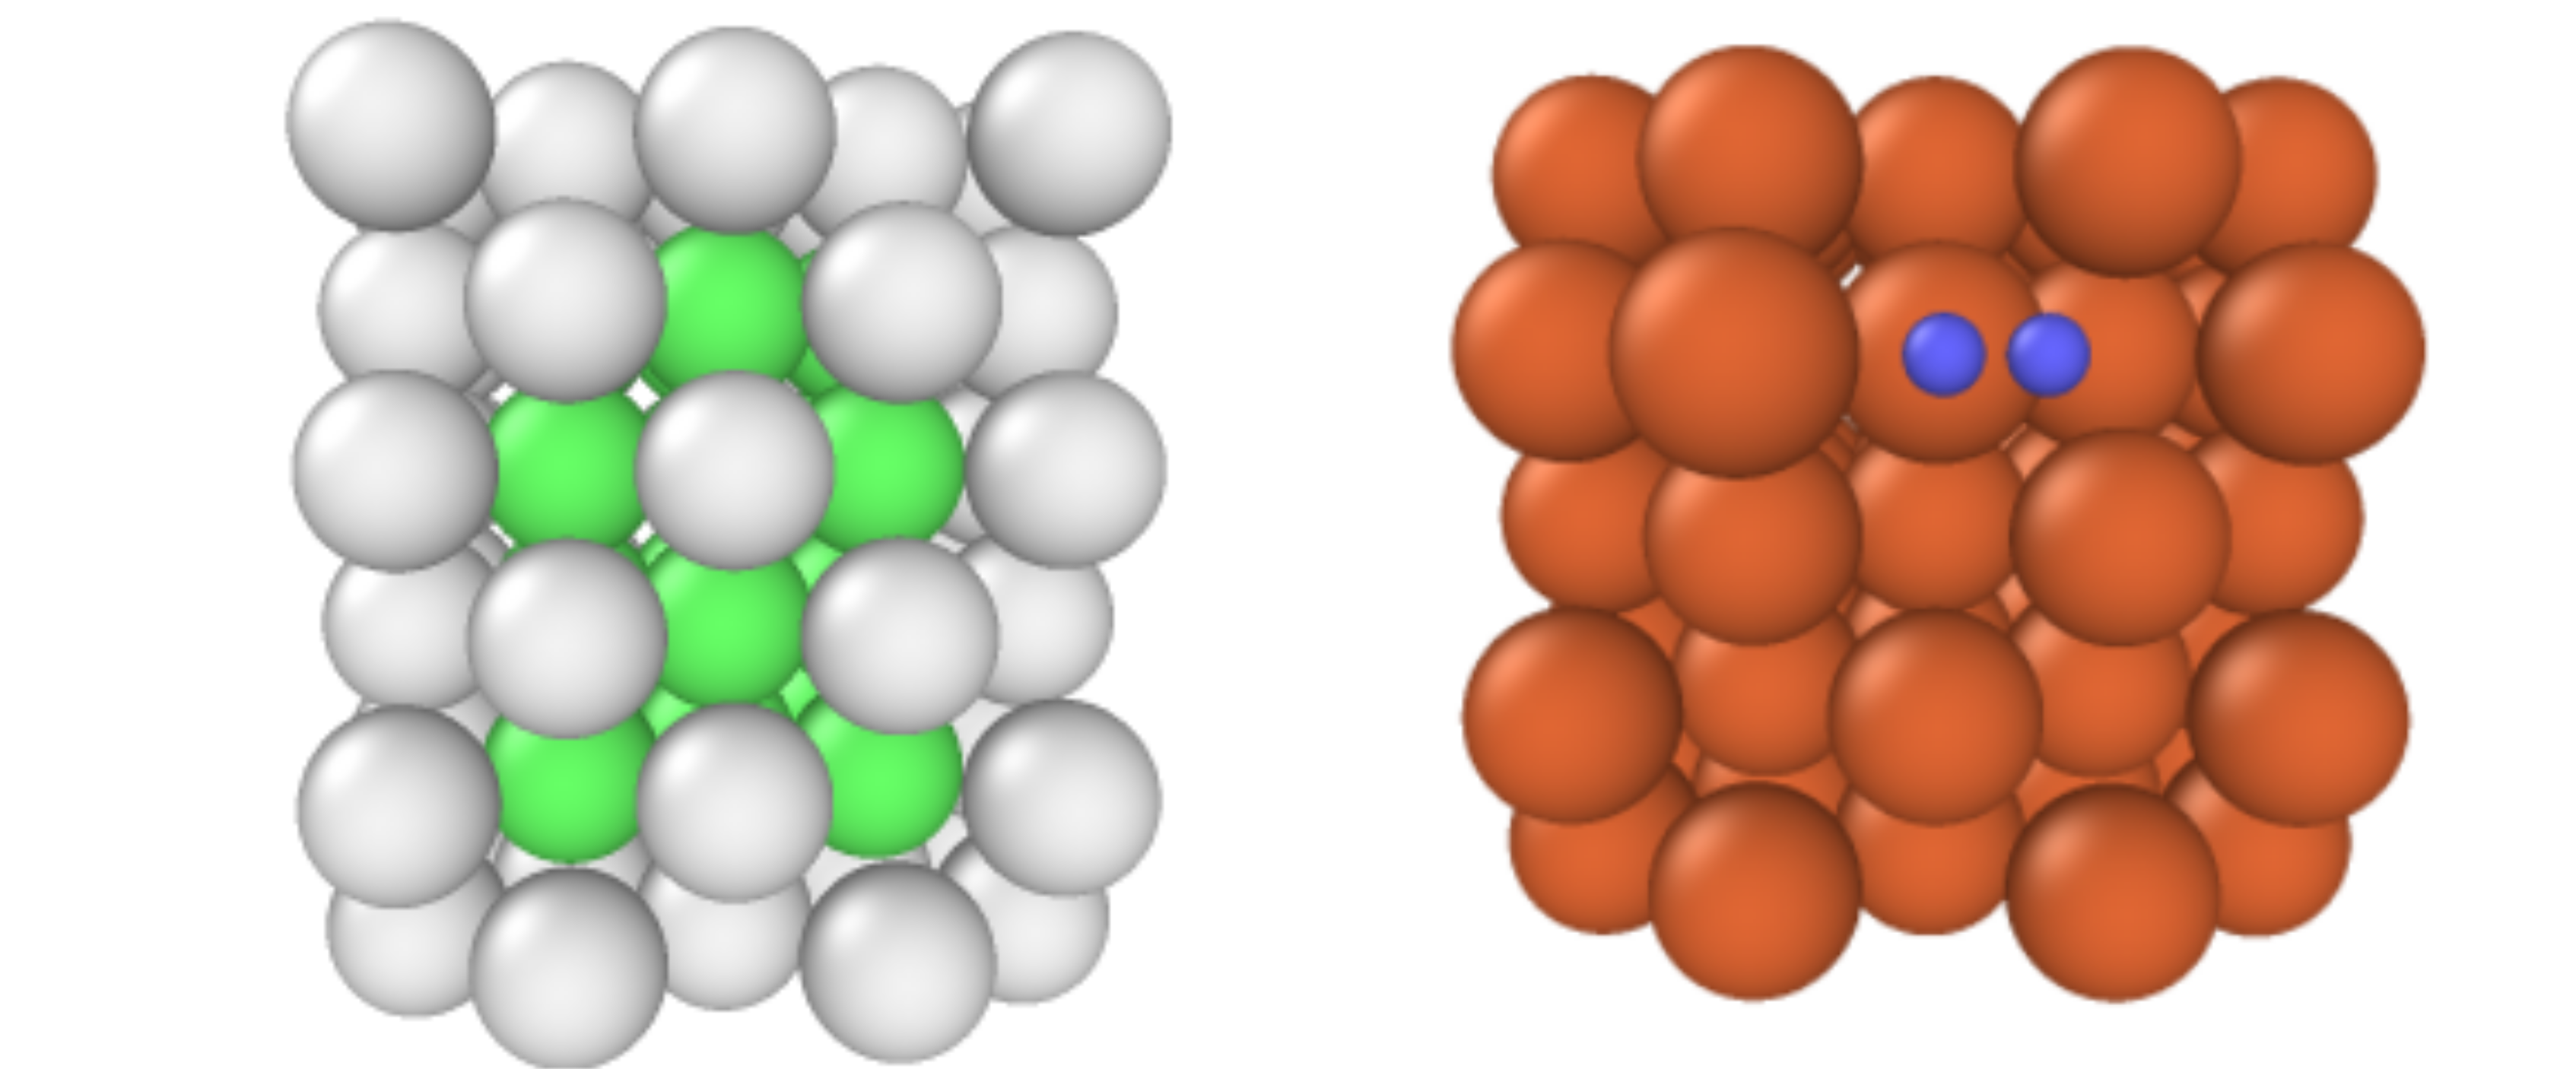
\includegraphics[width=\columnwidth]{./invariance/rec_examples/exrecal/combined.png}
\caption{(a) 75 atom cuboid cluster of face centered cubic (FCC) crystal. Green atoms are in an FCC environment, and have a complete
set of FCC neighbours, grey atoms are surface atoms of the cluster and a have a lower coordination number.
(b) Same cluster with an extra Ni atom and two additional atoms placed on the surface at two different sites. 
\label{fig:cuboid}}
\end{center}
\end{figure}
%
The density of states in Fig.~\ref{fig:fcc_dos} is computed using 11 levels of recursion: i.e, coefficients
are computed from $a_{0}$ to $a_{11}$ and $b_{0}$ to $b_11$. The Hamiltonian consists of five d orbitals.
The Hamiltonian parameters and the coefficients of the continued fraction are given in Table~\ref{tab:reccoeffs}.
The total DOS in this case is computed by summing up the continued fractions computed for each of the 
five starting orbitals. Symmetry considerations would allow this to be constraine to the two inequivalent 
orbitals $t_{2g}$ and $e_{g}$ however the finite cluster size will disrupt the symmetry of the recursion coefficients.
%
\begin{figure}
\begin{center}
{\graphicspath{{./invariance/rec_examples/exrecal/}}\input{./invariance/rec_examples/exrecal/recal_dos.tex}}
\caption{Top panel: the local density of states on the central atom for the Ni cluster in Fig.~\ref{fig:cuboid}
is computed. Bottom panel:  along with the contribution of the band structure to the cohesive energy and the integrated
density of states.\label{fig:fcc_dos}}
\end{center}
\end{figure}
%

\begin{table}
\begin{center}
\begin{tabular}{|c|c|}
\hline
$a_{n}$ & $b_{n}$ \\
\hline
 0.000000E+00 & 0.100000E+01\\
-0.736283E-02 & 0.295643E-02\\
-0.296524E-01 & 0.178593E-02\\
-0.126548E-01 & 0.221181E-02\\
-0.225989E-01 & 0.178256E-02\\
 0.296606E-02 & 0.141733E-02\\
-0.129493E-01 & 0.196435E-02\\
-0.136124E-01 & 0.141377E-02\\
-0.170328E-01 & 0.181703E-02\\
-0.161681E-01 & 0.173104E-02\\
 0.000000E+00 & 0.148088E-02\\
\hline
\end{tabular}
\caption{Coefficients for the continued fraction DOS for a $d_{xy}$ orbital of a Ni 
atom in the middle of a small nickel cluster.}
\end{center}
\end{table}

The difference in the qualities, in terms of the structure revealed, in the DOS 
is determined by the different termination scheme employed. 
\footnote{See the routines \texttt{DENCRS} and \texttt{DENSQ} 
for the square root and analytic terminator (TermDOS) schemes and \texttt{DENQD} 
for the QuadDOS termination scheme in the Cambridge Recursion Library 
\cite{nex84,haydock84,haydock85}.
The asymptotic behaviour of the continued fraction coefficients 
are affected by the presence of singularities
in the spectrum: e.g. delta functions near the band edges,the band edges
themselves, and Van Hove singularities.
There is considerable literature on the topic of termination schemes 
and the analytic structure of the asymptotic coefficients:
\cite{hodges77,bylander80,turchi82,haydock84,luchini87,glanville88,
yoshino87,yoshino88,haydock89,haydock10}.
In certain cases expressions for the behaviour of the coefficients
is given in terms of sinusoidal or elliptic functions linear prediction techniques
have also been used to study the behaviour of the recursion coefficients in the
asymptotic region \cite{allan84}. Given the rise of inference techniques in recent
years the latter approach may be worth some investigation.}

\subsection{Defects, Surface Electronic Structure and Orbital Peeling}
Surface catalysis is a topic of immense interest in chemistry and chemical engineering.
The rate at which reactions proceed is important in industrial and biomedical 
applications. The presence of a surface disrupts the periodicity required to use Bloch's theorem,
at least in the direction normal to the surface, and the in-plane periodicity is likely to 
be compromised by steps, vacancies and impurities, etc. along the material surface.
All this is to say that where there is a surface there is likely to be 
a need for recursion.

The need for a direct calculation of binding energy between adatoms or
the binding of a defect impurity in a lattice stems from the difficulties in computing 
these quantities via the method of energy differences. Performing two total
energy calculations on systems with $10^23$ atoms and subtracting the
resulting numbers is not a well conditioned problem. 
The very nature of the problem suggests that exploiting symmetries
will not greatly simplify things.

Relevant work on surfaces using the recursion method can be found in 
Refs.~\cite{haydock72, kelly73, kelly74, kelly74b, burke76, haydock79, haydock82}.
In particular \cite{haydock79} presents a semi-quantitative treatment of chemisorption of simple
molecules to transition metal surfaces across the transition metal series, 
a study which provides a strong positive example of analysis of homologous 
trends in materials according to Ehrenreich's fourth point (See Ehrenreich's
Points~\ref{en:ehrenreich} from Chapter~\ref{chap:intro}).
A detailed discussion of surface catalysis is also given in Ref.~\cite{haydock80}
for the dissociation of hydrogen on a transition metal surface. \footnote{The 
connection to embrittlement phenomenon will be discussed in detail in Chap.~\ref{chap:metallurgy}}.

The Cambridge Recursion Library provides an example 
to demonstrate some of the technique required to perform 
direct calculations of adatom interactions. The example treats the problem of the interaction of adatoms on a 
surface, i.e. adatoms interacting via the metallic substrate.
The formalism developed in Ref.~\cite{einstein73} allows for the study of adatom
interaction energy as a function of band filling, adatom energy level, and the hopping
potential chosen between the adatom and the substrate. The generalization
to multiple orbital adatoms was given in Ref.~\cite{burke76}. 

The problem reduces to finding the difference in the total energy of the system when
adatoms are distant (infinitely separated) and when they are close together.
The total energy of the system is written:
%
\begin{equation}
U_{\rm TOT} = \sum_{i}\epsilon_{i} - U_{\rm ES},
\end{equation}
%
the first term is the band structure contribution to the energy, integrated
across all the occupied electronic states (on an adatom), and the second term is the electrostatic
energy, including the interelectron repulsion (to avoid double counting), and the repulsion
between the ion cores. It is the first term that is considered to be of primary 
interest in the example and corresponds to the energetic contribution coming 
from the adatoms sharing electrons via the d-band substrate.

The calculation proceeds as follows. First the two atoms are placed at a sufficient
distance that they do not interact and the energy:
%
\begin{equation}
U_{1} = \int_{-\infty}^{E^{(1)}_{F}}EN_{1}(E)dE,
\end{equation}
%
is computed. 

Then the two adatoms are allowed to come together on the surface, 
a new density of states is recalculated along with the new Fermi level.
%
\begin{equation}
U_{2} = \int_{-\infty}^{E^{(2)}_{F}}EN_{2}(E)dE,
\end{equation}

The integrals of the two density of states up to the two Fermi energies are equal
(no electrons have been added to the system).

The interaction is now given:
%
\begin{equation}
W = \int_{-\infty}^{E_{F}} (E-E_{F})(N_{2}-N_{1}) dE
\end{equation}
%

The two reference systems are labeled System 1 and System 2. In Fig.~\ref{fig:burkesurf}
System 1 consists of two substrates each with an adatom, System 2 is a substrate with
2 adatoms and the empty substrate giving a Hamiltonian $H_{2}+H_{0}$.

The density of states then become:
%
\begin{equation}
N_{1} = 2{\rm Tr}[EI-H_{1}]^{-1}
\end{equation}
%
\begin{equation}
N_{2} = {\rm Tr}[EI-H_{2}]^{-1}
\end{equation}

Finally the identity: 
%
\begin{equation}
{\rm Tr}[EI-H]^{-1} = \frac{\partial}{\partial E} \log \det[EI-H],
\end{equation}
%
is employed to reach an expression for the difference in the density
of states $\delta N=(N_{2}-N_{1})$.
%
\begin{equation}
\delta N = \frac{\partial}{\partial E}\log\frac{\det[EI-H_{2}]}{\det [EI-H_{1}]}\frac{[EI-H_{0}]}{[EI-H_{1}]}
\end{equation}
%

What then follows is some consideration of the block structure of the matrices 
$H_2$, $H_1$ and $H_0$. $H_2$ is a partitioned matrix of dimension 
$5N+6$ and $H_1$ has dimension $5N+3$. $H_{0}$ is the substrate Hamiltonian 
with dimensions $5\times N$ (orbitals times atoms).
The self energy elements are given in the block $E_A$, $V_{1}$ and $V_{2}$ describe
the atoms interactions with the substrate and the $V_{12}$ describe the interaction
between adatoms. Some identities from matrix algebra employed in Ref.~\cite{einstein73}
and given in the appendix of Ref.~\cite{burke76} are then used to simplify the
expressions to:
%
\begin{equation}
\delta N = \frac{\partial}{\partial E}\log \frac{\det G_{1}}{\det G_{2}}
\end{equation}
%

The physical meaning is that $\log \det G_{2}$ gives the energy required to pull
one of two adatoms away from the substrate and its paired atom, the $\log \det G_1$
term is the energy required to put it back on substrate at an isolated site. 
The difference between these two energies is then the interaction energy. 
Formulating the problem as a matrix means the determinant can be split 
into a sum over five separate logarithms. This is accomplished by ``orbital peeling".

\begin{equation}
{\rm det}|G_{2}| = \bar{G}_{21}\bar{G}_{22}\bar{G}_{23}\bar{G}_{24}\bar{G}_{25}
\end{equation}

\begin{equation}
{\rm det}|G_{1}| = \bar{G}_{11}\bar{G}_{12}\bar{G}_{13}\bar{G}_{14}\bar{G}_{15}
\end{equation}

The matrix elements for each $G_{i\alpha}$ should be very familiar at this point:
%
\begin{equation}
G_{i\alpha}=\bra i,\alpha| [E-\bar{H}_{i\alpha}]^{-1} |i, \alpha\ket
\end{equation}
%
with $i=1,2$ $\alpha=1,5$. The matrix $\bar{H}_{i\alpha}$ is formed by taking 
$[E-\bar{H}_{i}]$, deleting the first $(\alpha-1)$ rows and columns 
to form $[EI-\bar{H}_{i\alpha}]$. The desired matrix element is now 
in the upper left-most corner of the matrix. 
Using this representation the difference in the density of states is calculated:
%
\begin{equation}
\Delta N = \sum_{\alpha=1}^{5} \frac{\partial}{\partial E}(\log\bar{G}_{1\alpha} - \log \bar{G}_{2\alpha})
\end{equation}
%

%
%The range of $E_{F}$ is restricted to $-0.068 \ge E_{F} \le 0.12$ Ryd by considerations
%based on the atomic configuration of tungsten as $5d^{4}6s^{2}$, meaning the band 
%should contain a minimum of 4 and a maximum of 6 electrons, with the band being half filled (5 e)
%considered the most plausible.

Fig.~\ref{fig:burkesurface} shows the energy difference as a function of the 
Fermi energy position. The energy is computed from the three p orbitals of a 
surface atom adhered to the same cluster studied in Sec.~\ref{sec:fccldos}.
%
\begin{figure}
\begin{center}
{\graphicspath{{./invariance/rec_examples/exorpeel/}}\input{./invariance/rec_examples/exorpeel/exorpeel.tex}}
\caption{Top panel: Adsorbate interaction energy as a function of the Fermi energy for a representative d band
substrate. Mutual interaction of the adsorbates is mediated by the substrate and the p-d surface interaction.
Interaction goes to zero when the substrate band is completely filled. 
Bottom panel: Difference in the total energy for the two adsorbate configurations as a function of
d-band filling (position of the Fermi energy). See Ref.~\cite{burke76} for details. \label{fig:burkesurface}}
\end{center}
\end{figure}
%

These early surface calculations using the recursion method were overwhelmed 
by a number of uncertainties. The lack of a procedure for a choice of the tight-binding 
Hamiltonian and accessing the self consistent charge density
in the presence of a surface being the most significant.
\footnote{For early work on Wannier functions at surfaces Ref.~\cite{smith74}. Also see 
\cite{mostoller79} for a treatment of surface effects using the recursion method.}
First principles work has greatly simplified access to these quantities and should remove 
some of the ambiguities in mapping ab initio data onto a local picture
of the electronic structure at surfaces. These advances mean that the 
recursion techniques described in Refs.~\cite{burke76, haydock79, haydock81} 
might be revisited with potentially profitable effect.

For applications of orbital peeling to defects and the 
computation of interaction energies and variations in the charge density
see Refs.\cite{gibson93,gibson94}. However that work partially relies 
on the computation of off diagonal of the Green's function. A topic
to which we turn now.

\subsection{Off-Diagonal Elements of the Green's Function}
The off-diagonal elements of the Green's function can be written:
%
\begin{equation}
G_{AB}(E) = \bra \phi_{A}|[H-E]^{-1}|\phi_{B}\ket,
\end{equation}
%
and they contain a lot of useful information. 

These off-diagonal elements are required to calculate 
response functions, \cite{terakura78}, interatomic 
forces \cite{finnis84, finnis87, ohta87}, and bond orders 
\cite{coulson39,tersoff86,pettifor89}.

One direct route to computing an off-diagonal elements of the Green's function
is by expressing it as a linear combination of two diagonal elements. 
This can be seen by forming new starting vectors 
from the potential linear combinations of $\phi_{A}$ and $\phi_{B}$:
%
\begin{align}
\phi_{+} = \frac{1}{\sqrt{2}}(\phi_{A} + \phi_{B})\\
\phi_{-} = \frac{1}{\sqrt{2}}(\phi_{A} - \phi_{B})\\
\phi_{i+} = \frac{1}{\sqrt{2}}(\phi_{A} + i\phi_{B})\\
\phi_{i-} = \frac{1}{\sqrt{2}}(\phi_{A} - i\phi_{B}),
\end{align}
%
we can retrieve the off-diagonal elements by computing 
two `normal' diagonal elements from these linear combinations.
For example, for an Hermition $\hat{H}$, and real $\phi_{A}$ and $\phi_{B}$ 
the $AB$ off-diagonal element of the Green's function can be computed as:
%
\begin{equation}
\label{eq:offdiaggreen}
G_{AB}(E) = \frac{1}{2}[G_{++}(E)-G_{--}(E)].
\end{equation}

To see how the off-diagonal elements contribute to the force on an 
atom we follow Sec. 2.4 of Sutton \cite{sutton88} and Ohta \cite{ohta87}.
First we reproduce their expression for the bond energy:
%
\begin{equation}
\label{eq:tbenergy}
u_{ij} = u^{\rm rep}_{ij} - \frac{4}{\pi}\sum_{\lambda\mu} 
h_{ij}^{\lambda\mu}{\rm Im}\int_{-\infty}^{\epsilon_{F}}G_{ji}^{\mu\lambda}(\epsilon+i0)d\epsilon,
\end{equation}
%
The total energy is then a sum over the bond energies:
%
\begin{equation}
\label{eq:tbtoten}
U^{\rm tot} = \frac{1}{2}\sum_{ij,(i\neq=j)}u^{\rm tot}_{ij}
\end{equation}
%

The expression for the bond force follows naturally as the gradient of the bond energy:
%
\begin{equation}
\label{eq:tbforce}
f_{ij}^{\alpha} = f^{\rm rep}_{ij\alpha} - \frac{4}{\pi}\sum_{\lambda\mu} 
\nabla_{i\alpha}h_{ij}^{\lambda\mu}{\rm Im}\int_{-\infty}^{\epsilon_{F}}G_{ji}^{\mu\lambda}(\epsilon+i0)d\epsilon,
\end{equation}
%
$\alpha$ is a Cartesian direction, $i,j$ are site indices, and $\lambda, \mu$ are orbital indices 
the z axis lies along the bond connecting atoms i and j. The first term in Eq~\ref{eq:tbforce} 
we will come back to this term in Chapter~\ref{chap:gw} and Chapter~\ref{chap:wannier}. 
It is very much a term determined by craft and describes the repulsive contribution of the ion cores. 
But all this to come. 

For now it is the second term that is of interest and
it is easily recognized as something we can access via the Green's function 
computed using recursion techniques. It is also important to note that 
Eq.~\ref{eq:tbforce} is certainly not a two body interaction! The Green's function 
as it is calculated accounts for information from every shell of neighbours 
until there are no more or the recursion process is terminated. 
The importance of this local formulation of forces should not be underestimated.
Many of the practical applications discussed in Chapter~\ref{chap:metallurgy} 
will rely on it.

%
These off-diagonal elements are also required to determine the vibrational properties. 
If we want the interatomic force constants in the harmonic approach we follow Finnis and
go to second order in the variation of the total energy to derive the interatomic force
constant matrix:
%
\begin{equation}
\label{eq:tbdynmat}
\psi_{\alpha\beta}^{ab} = \hat{\psi}_{\alpha\beta}^{ab} +  \sum_{dnq\sigma}(\delta 
\rho_{bd,a\alpha}^{nq,\sigma}\nabla_{\beta}h_{db}^{qn} + \delta\rho_{ad,b\beta}^{nq,\sigma}\nabla_{\alpha}h_{da}^{qn}),
\end{equation}
%
$h^{qn}_{db}$ is a two center hopping integral that links the orbital n on atom b to orbital 
q on atom d. For the d electrons this integral is taken to decay as
$\r^{5}$. The density changes are proportional to the variation in the Hamiltonian 
time the response function. Displacing atom a in the $\alpha$ direction induces a change in the
bond charges about atom b. The change in the bond charge between atoms b and d 
in the spin-$\sigma$ channel stemming from orbitals n and q is given by:
%
\begin{equation}
\label{eq:tbdeltarho}
\delta \rho_{bd,a\alpha}^{nq,\sigma} = \sum_{cmp}(\chi_{bc,ad}^{np,mq,\sigma}+\chi_{ba,cd}^{nm,pq,\sigma})\nabla_{\alpha}h_{ac}^{pm}
\end{equation}
%
where the response function is defined as:
%
\begin{equation}
\label{eq:tbresponse}
\chi_{bc,ad}^{np,mq,\sigma} = \frac{1}{\pi}{\rm Im}\int^{E_{F}}G_{bc}^{np,\sigma}(\epsilon)G_{ad}^{mq,\sigma}(\epsilon)d\epsilon,
\end{equation}
%

An interesting relationship can be derived between off-diagonal elements
and the response functions \cite{terakura82, sutton88}:
%
\begin{equation}
\frac{dG}{dE}=-G^{2},
\end{equation}
%
and upon integration:
%
\begin{equation}
\frac{-2}{\pi}G_{jk}(E^{+}) = \frac{2{\rm Im}}{\pi}\int^{E}\sum_{l}G_{jl}(E')G_{lk}(E')dE'.
\end{equation}
%

Fig.~\ref{fig:tbresponse} gives a pictorial representation of some of these many indiced terms. In 
Ref.\cite{finnis84} the Green's functions are computed out to sixth nearest neighbour. This allows
for force contributions out to the thirteenth nearest neighbour. Symmetry relations are exploited 
in that work to reduce the number of unique off-diagonal Green's function elements to 
33 separate functions which are tabulated and used to compute the force constant matrix. 
%
\begin{figure}
\begin{center}
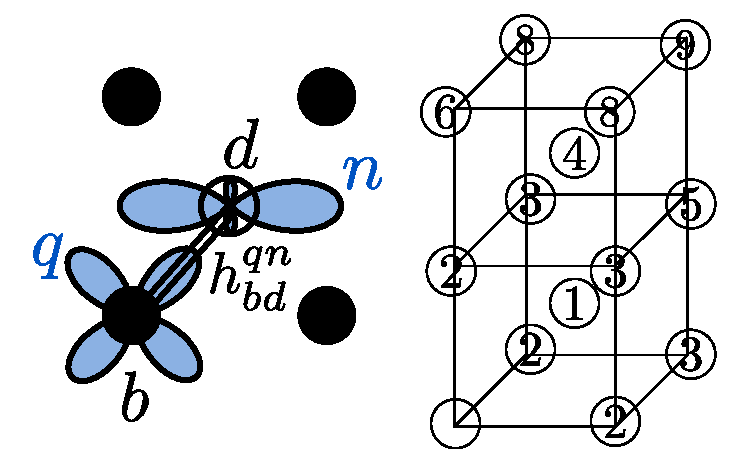
\includegraphics[scale=0.8]{./invariance/tbresponse.pdf}
\caption{Pictorial representation of the terms and sites described by Eq.~\ref{eq:tbdynmat}.
On the left atoms $b,d$ and two orbitals centered on those sites, $n, q$, and the energy
integral $h_{bd}^{qn}$ which connects them. On the right are two unit cells
of BCC crystal with the nearest neighbours to the zeroth atom labeled out to its sixth nearest
neighbour.\label{fig:tbresponse}}
\end{center}
\end{figure}
 

The type of analysis in Ref.~\cite{finnis84} is taken as an example
of the desired model computational framework these notes pursue. 
The approach satisfies many of Ehrenreich's points ~\ref{en:ehrenreich}: 
direct experimental links \cite{powell68, colella70, shaw71}, 
tractable calculations for a minimally idealized system, and, most importantly, 
the calculations have {\emph explanatory and predictive power 
across a homologous series}, in this case the BCC transition metals.
\footnote{The mystery of obtaining a good experimental phonon spectra in published
literature continues... A. M. B. G. De Vallera, Ph.D. thesis, Cambridge University, 1977 (unpublished).
However it is apparently quite similar to NbMo\cite{powerll68}.}

The only point not fully satisfied is that of theoretical justification.
The force constants as determined in Eq.~\ref{eq:tbdynmat}
rely on the repulsive force and some means of determining 
the local Hamiltonian i.e. its bond integrals and their 
radial dependence {\it ab initio}. Addressing this issue 
will be the subject of subsequent chapters. For the present we can simply 
admire how the formalism can yield results entirely in keeping with local 
notions of forces and electron orbitals.
 
Eqs.~\ref{eq:tbdynmat, eq:tbdeltarho, eq:tbresponse} encode
a huge amount of information. Although well developed reciprocal space 
techniques exist, see Ref.~\cite{baroni01}, to obtain the phonon dispersion
curves, the local formulation still has a great deal of 
interprative value, and crucially, will remain valid
in situations where Bloch's theorem does not.

The bond order between atoms has a long history
beginning with Coulson's study of carbonyl 
chains in Ref.~\cite{coulson39}. It is a good exercise to compare
the derivative of Eq.~\ref{eq:tbtoten} with respect
to the hopping integral and the Green's function,
with Coulson's definition of the bond order.

The order of a given bond is a measure
of the force tending to change the length of a given bond
for small variation of the bond length.

The more frequently referred to bond order, defined
in terms of Green's functions, is the integrated 
energy difference between a symmetric 
and anti-symmetric combination of nearest neighbour 
orbitals \cite{pettifor89}:
%
\begin{equation}
\label{eq:bondorder}
\Theta_{ij} = - \frac{2}{\pi} {\rm Im} \int^{E_{F}}\left[G^{+}_{00}(E)-G_{00}^{-}(E)\right]dE.
\end{equation}
%
The bond order in this form then appears like a measure of the interference 
between orbitals on the two sites.

As we integrate up in energy the difference in the symmetric and antisymmetric 
combinations of the two states are accumulated. The resulting integral is 
then a scalar which measures the sign and magnitude of the
interference between the two localized orbitals up to the Fermi energy.

Eq.~\ref{eq:offdiaggreen} gives an immediate scheme for computing the off-diagonal
elements but can result in the need for substracting two largish quantities to find
a small one. Such a procedure is never ideal. This concern and others motivated the introduction
of the block recursion method which will be discussed in the next section.

First though a small digression.

Harrison in his textbook argues that every conclusion drawn in his work follows immediately
from the proposition that electrons are simultaneously a particle and a wave. This is
somewhat abstract. In the present context we can propose a tentative meaning to this:
the electron is a particle when we can point to it and say there it is in that orbital
centered on that atom, it becomes a wave when the recursion is iterated and the localized 
orbital spread outwards and interact with the space around it. 
The form this interaction takes in the recursion method is the linear mixing of
the other localised vectors in the system with varying coefficients from further and further away. 
Adding these vectors together is equivalent to allowing them to interfere constructively or 
deconstructively. 

At the end the recursion method gives a record of the projection of 
the starting orbital on to each of its increasingly distance neighbours 
as a function of energy. The electron, though confined to a 
single energy and a single state on the lone atom, when in a solid, 
can take on a range of shapes across a range of energies distributed 
throughout a crystal.

\subsection{Non-Orthogonal Recursion}
The underlying assumption about the basis vectors
used to describe the system up to this point have 
been that they are orthogonal. When this is not the case some
choices need to be made. There are two options.
The most tempting option is just to ignore the non-orthogonality 
of the vectors and carry on.
The other is to modify our approach somewhat. 

The latter course is the morally upright one. The problem
of non-orthogonality of basis vectors is closely connected
to the Block Recursion method which we will come to in the 
next section. But the ideas underlying non-orthogonal 
recursion calculations are a bit simpler and should
be treated first. 

\subsubsection{Two Sided Lanczos}
For the case where $H\neq H^{*\dagger}$ i.e. for a non-Hermitian
Hamiltonian a two-sided Lanczos algorithm exists as discussed in
Ref.\cite{haydockkelly75} following Wilkinson's description.

Two starting vectors are chosen $|u_{0}\ket=|0\ket$, $|v_{0}\ket=|0\ket$
and two chains of recurrences are generated:
%
\begin{equation}
b_{n+1}|u_{n+1\ket = H|u_{n}\ket - a_{n}|u_{n}\ket - b_{n}|u_{n-1}\ket
\end{equation}
%
\begin{equation}
b_{n+1}|v_{n+1\ket = H^{\dagger}|v_{n}\ket - a_{n}|v_{n}\ket - b_{n}|v_{n-1}\ket
\end{equation}
%
where $a_{n} = \bra v_{n}|H|u_{n}\ket = \bra u_{n}|H^{\dagger}|v_{n}\ket$
and the overlap is computed  $b^{2}_{n+1} = \bra v_{n+1}|u_{n+1}\ket$.

The danger of the two sided recursion algorithm is that the inner
product of the vectors $\bra v_{n+1}|u_{n+1}\ket$ could become negative.
The density of states would no-longer be non-negative which makes it
more difficult to interpret. The fact that the Hamiltonian is non-Hermitian
does not guarantee this will be the case so the application of this
method may not produce any complex eigenvalues.

\subsubsection{Gauss-Siedel Overlap}
The approach to the non-orthogonal basis vectors taken in the 
\texttt{CamRecLib} routine \texttt{recno} is slightly different.
It is similar to the approach taken in Refs.\cite{jones84} which
uses the Gauss-Siedel method to efficiently incorporate the nonorthogonality.
Following the notation in \cite{nex89}

The eigenvalue problem to be solved is:

\begin{equation}
MX=\epsilon S X
\end{equation}

The actual Greenian computed is:
%
\begin{equation}
U^{T}S(S\epsilon-M)S^{-1}U
\end{equation}
%

The Gauss-Siedel Algorithm is used to compute the application of the inverse 
of the overlap matrix to the recursion vector $S^{-1}\psi_{n+1}$:
\begin{equation}
U_{n+1}^{i} = \psi_{n+1} - LU_{n+1}^{i} - RU^{i-1}_{n+1}
\end{equation}

with L and R are the strict left and right triangular parts of S. The
efficiency of the algorithm is determined by how diagonally dominant
matrix S is. 


\subsection{Block Recursion}
By picking a single orbital and turning the wheel on the recursion method a
chain of coefficients and vectors can be generated. However rounding errors in the evaluation
of the matrix vector products mean the accumulation of numerical noise
generated by the artifical truncation of the recurrence
can disrupt underlying symmetries. This can be demonstrated where there are 
deviations in the density of states computed for a given orbital if the z-axis 
is changed arbitrarily which should not be the case. This provided one motivation for 
the block recursion method. 

The block recursion method is a direct and intuitive extension of the scalar method.
In this method a {\emph set of m} initial orbitals are chosen. The recursion
coefficients become matrices. The technique and its implementations are described 
in Refs.~\cite{jones84, legrand85, inoue87, nex89, godin91, ozaki00}. For discussions
on the implementation and applications of the block recursion method see
the computation of the local electron density in a system by 
Lewis and Jones in Ref.~\cite{jones84}, Paxton's study of the
stability of different phases of silicon in Refs.~\cite{paxton87, paxton88}. The work of 
Godin and Haydock on the passage of electrons through disordered media 
in Refs.~\cite{godin86, godin88}.
The notation we supply here is a synthesis of the descriptions given in
Refs.~\cite{paxton88, nex89, godin91} and is in accord with the accompanying CamRecLib
routines.

The asymptotic behaviour of the recursion co-efficients in the scalar recursion case
is analyzed in \cite{turchi82, yoshino87, yoshino88, haydock10, alhaidari18}.

If a small discursion into metaphor is allowed we might suggest 
the difference between the scalar recursion and the block recursion method is 
similar to the difference between playing a number of notes at the 
same time like a musical chord rather than picking out single notes at 
a time as in a melody.

%T.J. Godin, Ph.D. Thesis, University of Oregon (1988).

\subsection{Phonon Recursion}
With a simple modification phonon spectra can be computed directly 
using the recursion technique. Instead of localized orbitals, localized 
displacements are introduced, and in the place of on-site and hopping
matrix elements force constants connect nearest and next 
nearest neighbour displacements. 
The papers and PHD thesis of Meek describes in detail the 
application of the recursion method to the computation of 
vibrational spectra \cite{meek76, meek78}. Electron-phonon coupling has also been
considered in this context\cite{terakura78}. The method is particularly useful for
computing vibrational spectra in disordered media 
where a statistical averaging procedure needs to be undertaken \cite{mookerjee04}.

The force constant matrix of a crystal can be written as:
%
\begin{equation}
\label{eq:forceconstant}
\Phi_{\alpha\alpha'}(l\kappa,l\kappa') = \frac{\partial^{2}V}{\partial u_{\alpha}(l\kappa) \partial u_{\alpha'}(l'\kappa')}
\end{equation}
%

The equation of motion for atom $i$ becomes:
%
\begin{equation}
m_{k} \frac{\partial^{2} u_\alpha (l\kappa)}{\partial t^{2}} = - \sum_{l'\kappa'\alpha'}
\Phi_{\alpha\alpha'}(l\kappa,l'\kappa')u_{\alpha'}(l'\kappa'),
\end{equation}
%
l, $\kappa$, and $\alpha$, represent the unit cell index, basis atom, and 
cartesian coordinate of the displacement respectively.

A solution of the form:
%
\begin{equation}
u_{\alpha}(lk) = \frac{1}{\sqrt{m_{k}}} U_{\alpha}(\kappa;\k)e^{[i(\k\cdot x(l) - \omega_{\k}t)]},
\end{equation}
%
is assumed where $U_{\alpha}(\kappa;\k)$ is the amplitude of the displacement.
%
\begin{equation}
\omega^{2}(\k) U_{\alpha}(\kappa, \k) = \sum_{\kappa'\alpha'}D_{\alpha\alpha'}(\kappa\kappa';\k) U_{\alpha'}(\kappa',\k)
\end{equation}
%
and the Fourier transform of the dynamical matrix has been introduced:

\begin{equation}
D_{\alpha\alpha'}(\kappa\kappa';\k) = \frac{1}{\sqrt{m_{k}m_{k'}}} \sum_{l'} \Phi_{\alpha\alpha'}(l\kappa,l'\kappa') e^{[i\k(x(l')-x(l))]}
\end{equation}
%
The vibrational frequencies of the normal modes of a cluster or crystal can then be determined 
from the secular equation:
%
\begin{equation}
{\rm det}|D(\k) - \omega^{2}(\k)I| = 0
\end{equation}
%

The Green's function matrix elements for the vibrational problem 
becomes the projection of the interaction matrix on to the 
displacement of atom $i$ in direction $\alpha$.
%
\begin{equation}
G_{i\alpha,i\alpha}(\omega^{2})= \bra i\alpha| \left[D- \omega^{2}I\right]^{-1} |i\alpha \ket
\end{equation}
%

For instance for 2 atoms in a unit cell of a perfect 
crystal Eq.~\ref{eq:phonon} would only
need to be computed for 6x6 matrix at every $\k$ point 
in the Brillouin zone to determine the vibration spectrum. 
In this case there would be little need for employing a recursion method.
Well developed techniques exist to obtain the force constant 
matrix at every $\k$ point from first principles \cite{baroni01}, 
however this again requires an assumption about
microscopic periodicity which may not be valid. For any amount of 
disorder at the atomic level, for instance in the CRN systems 
studied by Meeks secular determinants of $3N\times3N$ with
$N=200-300$ may need to be solved. In these situations recursion 
type calculation become necessary.
%
\begin{figure}
\begin{center}
{\graphicspath{{./invariance/rec_examples/phonon/}}\input{./invariance/rec_examples/phonon/phonon_dos.tex}}
\caption{The local phonon density of states for a small six atom molecule 
composed of two atom types. The model is specified by giving the 
masses of the two atoms. In the present simulation 
the masses are chosen to be 0.25 and $0.189$ amu. Two force constants are also
specified, a bond stretching force constant of 1.0, 
which is the same for both atomic types
and two bond bending force constants of 0.5 and 0.25 \label{fig:phonondos}. 
The phonon DOS relies on the routine
\texttt{RECSUM} to combine the continued fraction coefficients 
for the vibration modes computed for each site. 
The six atom system has $3N-6=12$ vibration modes and the 
DOVS integrates to 12 as expected.}
\end{center}
\end{figure}
%
The phonon density of states and the integrated phonon density of 
states is depicted in Fig.~\ref{fig:phonondos} 
for a six atom molecule consisting of two atomic types. The number of 
sets of continued fraction coefficients
that needs to be generated is equal to $3*N_{s}$ where $N_{s}$ 
is the number of atoms that the phonon LDOS
or density of vibrational states (DOVS), is computed 
for and the factor of 3 is for the displacement in each 
atomic direction. The expression for the average phonon density of states
over the different matrix elements of the resolvent 
is first over the cartesian displacements $\alpha$:
%
\begin{equation}
n_{i}(\omega^{2}) = \sum_{\alpha}n_{\alpha,i}(\omega^{2}),
\end{equation}
%
\begin{equation}
N(\omega) = \frac{2\omega}{N_{s}}\sum_{i}^{N_{s}}n_{i}(\omega^{2}),
\end{equation}
%
its integral gives the total number of vibrational modes.

In Fig.~\ref{fig:phonondos} two sites are used to generate the 
DOVS, to a depth of $7$ in the continued fraction coefficients. 
The postprocessing of the continued fraction coefficients 
is the same as in the case of the surface and bulk DOS calculations. 
In Meeks work sufficient feature resolution in the DOVS is 
achieved with a depth of 20 in the recursion steps for a 
cluster of 344 diamond atoms. The force constants entering 
these models were not ab initio instead being 
derived from a model due to Born \cite{born14}. 
It is now possible to obtain highly accurate force 
constants from first principles. The higher 
quality force constant matrices that can be generated 
as a result could well be reflected in the quality 
(with respect to experiment) of the features 
observed in the density of states.

Direct examination of the routines involved in the 
computation of the Phonon DOS itself give a good feeling 
for how the recursion method works. In Table~\ref{tab:phonon} 
the various routines and the task they accomplish are listed. 
These routines specify the entire problem and with minor 
adaptations, (the crystal structure, force constants etc.), can 
be used to compute the DOVS for any system.

\begin{table}
\begin{small}
\begin{tabular}{|l|l|}
\hline
Routine & Task \\
\hline
\texttt{EXPHNDS} & Generate Recursion Coefficients for DOVS \\
\hline
\multicolumn{2}{|c|} {Define and Initialize Force Constant Matrix} \\
\hline
\texttt{SCAN} & Loop Over Atoms in Cluster Calling \texttt{DMGEN}. \\
\texttt{DMGEN} & Compute the Dynamical Matrix between Atoms (According to Ref.~\cite{meek}.) \\ 
\texttt{RECAL} & Compute Chain Coefficients via Recursion Algorithm. Hamiltonian applied using \texttt{DMHOP}. \\
\texttt{DMHOP} & Satisfies requirements of RECAL calling \texttt{MLT} to apply dynamical matrix at each step. \\
\texttt{MLT} & Computes and Accumulates Product of Dynamical Matrix at Atom I with a Displacement. \\
\texttt{EXPHNPLT} & Reads Recursion Coefficients and Tabulates DOVS \\
\hline
\multicolumn{2}{|c|} {Tabulate DOVS and Integral of DOVS} \\
\hline
\texttt{RECSUM} & Compute Sum of Densities ($N_{S}*3$) and Store the Resulting Recursion Coefficients \\
\texttt{DENQD} & Evaluate DOVS and Integral of DOVS Using Quadrature\\
\hline
\end{tabular}
\end{small}
\caption{The subroutines required to perform a typical Local Density of Vibrational 
States (DOVS) calculation. \label{tab:phonon}}
\end{table}

For other examples of the computation of vibration spectra the stretching modes 
in ice have also been studied using the recursion method\cite{mcgra78,bergren82}.

The actual computation of forces using the recursion method is possible. 
A discussion of the computation of forces in tight binding bond models can be found in
Ref.~\cite{sutton88} and explicity expression using the recursion method can be found in 
\cite{boswarva82, boswarva87}. However it should be noted that obtaining ab initio forces
is now a highly developed technique and populating a force constant matrix for a recursion
type calculation in novel alloys and chemical environments would be an interesting application
of the method.

\footnote{For an instructive derivation of the solution to an infinite 
chain, using classical mechanics, of spring coupled massed using a continued fraction expansion see 
The Classical Harmonic Chain: Solution via Laplace Transforms and Continued Fractions 
(https://arxiv.org/pdf/1608.00616).}

\section{Chains and Moments}
Before concluding this chapter there are a few 
pictorial and heuristics comments on the recursion method
and related methods.

The recursion method produces the eigenvalue spectrum
for a given Hamiltonian. The idea of a particle exploring
the space around it according to the rules of the Hamiltonian
can be formulated as excursions from a starting orbital localized
on some atom. As the electron (or phonon) hops from atom to atom
new eigenstates of the system are uncovered.

The second trend in the literature for producing the density of states
from a locally defined Hamiltonian was to expand the density of
states in terms of its moments. This can be seen by expanding the
Green's function as a geometric series in the energy and the Hamiltonian.
The comparison is valuable because it leads to the interpretation of 
the recursion method as producing a density of states by closed walks
from a starting point.\cite{ducastelle70} 
Expanding the Green's function gives:
%
\begin{equation}
[E-H]^{-1} = \sum_{n=0}^{\infty} \frac{H^{n}}{E^{n+1}}.
\end{equation}
%

The $r^{\rm th}$ moment of the local density of states can be written:
%
\begin{equation}
\mu^{r} = \int E^{r}N(E)dE = -\frac{1}{\pi}{\rm Im}\sum_{n=0}^{\infty}\int E^{r}\bra 0|\frac{H^{n}}{E^{n+1}}|0\ket dE.
\end{equation}
%

When $H$ is a strictly local Hamiltonian the only non-zero matrix elements 
will be immediate neighbours of the starting orbital $0$. The means
the matrix element can be written as a over closed paths of length $r$:
%
\begin{equation}
\label{eq:circuit}
\bra 0|H^{n}|0 \ket = \sum_{i,j,k,...}\bra 0|H|i\ket\bra i|H|j\ket\bra j|H|...\ket\bra 1|H|0\ket,
\end{equation}
%
0ijk...10 is a closed circuit through the lattice. Any circuit that takes hops between sites 
that aren't connected by the Hamiltonian won't make any contribution to the matrix element
in Eq.~\ref{eq:circuit}.

Detailed workings of the application of the recursion method to a surface atom in Cubium
are presented in Ref.~\cite{haydock75}. 

\section{Future Work}
The references provided here and in Vol. 35 demonstrate the impact of 
the recursion method already achieved by 1980. Only a small subset of that 
work have been referenced here. The ability of the tight binding framework 
to provide an explanatory model for trends in homologous materials is 
well demonstrated by the work on the crystal structure along the transition
metal series \cite{pettifor70}, the Chevrel Compounds of Molybdenum Chalcogenides Ref.~\cite{bullet77}.
The recursion formulation of the tight binding method was used to order
the structures of the compounds in the Lave phases in Ref.~\cite{johannes76},
and explaining trends in surface chemistry by determining 
the heat of adsorption for simple molecules transition metals across 
the row of the transition series in \cite{haydock78}. 

A perturbation theory built on the recursion method has also been formulated
making it possible to study photoemission phenomena \cite{mclean77}. 
The use of the recursion method to compute susceptibilities has also been addressed, 
see for instance Ref.~\cite{terakura78}, both these applications will be further 
elaborated on in Chap.~\ref{chap:manybodyrec}.

The conclusion to Haydock's chapter in that volume is interesting in he gives 
prognosis for further work along two lines. 

The first line of research consists of diffusing quantum processes in disordered
solids:
%
\begin{quote}
One of the outstanding problems is that of the Anderson model
of a disordered solid. Here the Hamiltonian is defined statistically and
one would like to transform to a corresponding statistically defined chain where
one could discuss the distributions of various physical quantities.
\end{quote}
%

The second line of inquiry consists of the extension of the recursion from a single 
particle description of electronic structure to a many-body Hamiltonian.
%
\begin{quote}
Finally, the reader may have noticed that the approach of this chapter has been entirely directed
toward independent particle models. However, many-body Hamiltonians must be similarly 
transformable to chain models. Aside from a small amount of thought and continuing interest, 
nothing has been done about this and it remains a most interesting problem concerning recursive 
solutions of the Schrodinger equation.
\end{quote}

	Since Vol. 35 was published there has been a rise in the accessibility of density functional methods 
and access to good single particle approximations to the electronic eigenstates of a crystal
is routine. Additionally, progress on the problem of determining the localized Wannier functions, 
means tight binding Hamiltonians can be determined unambiguously.

First principles understanding of Green's function methods and their application to the many body
problem have also developed. In the following chapters we will look at how these developments
coupled with recursion techniques can provide a framework for a computationally tractable 
toolkit for performing highly accurate calculations of material properties.

\section{Questions}
\begin{itemize}
\item (Kwidzinski: Continued Fractions and Classical Vibrations) 
      Let $x_{n}(t)$ be a time dependent function for the position of mass $m$.
      For a one sided infinite chain of coupled harmonic oscillators, with 
      spring constants $k$ and masses $m$ the equations of motion for the $0^{\rm th}$ and
      $n^{th}$ spring can be shown to be:
      %
      \begin{equation}
      (s^{2} + \frac{k_{0}}{m_{0}}) x_{0}(s) - \frac{k_{0}}{m_{0}}x_{1}(s) = As 
      \end{equation}
      %
      and for the $n^{th}$ oscillating mass:
      %
      \begin{equation}
      (s^{2}+\frac{k_{n-1}+k_{n}}{m_{n}})x_{n}(s)-(\frac{k_{n-1}}{m_{n}}x_{n-1}(s) + \frac{k_{n}}{m_{n}}x_{n+1}(s)) = 0
      \end{equation}
      % 
      where $x_{m}(s) = \int_{0}^{\infty}e^{-st}x(t)dt$ is the Laplace transform of the time dependent position.
      Write this system of equations as a matrix where the vectors 
      are $[x_{0}(s), 0, 0, 0,...]^{\rm T}$, $[0, x_{1}(s), 0, 0, ...]^{\rm T}$ etc,
      and use the determinant expansion trick in Eq.~\ref{eq:cauchy} to find a 
      continued fraction expansion for the $x_{0}$ element.
      Simplify this continued fraction to obtain an expression for the Laplace 
      transform of the position operator.
      %
      The time dependence of the position can then be found by performing the inverse Laplace transform
      this can be done most easily by checking a correspondence table
      in an appropriate handbook. (For instance, M. Abramowitz, I. Stegun (1965) 
      Handbook of Mathematical Functions).
      %Should give the first bessel function.
      %For a two sided infinite chain the relevant equations of motion are: 
      %What is the continued fraction expansion for the laplace transform of a mass $n$?
      %What is its form in the time domain?

\item (Haydock: Recursion for a Free Electron) Take the Hamiltonian for a non-relativistic 
free electron in radial coordinates:
%
\begin{equation}
H = \frac{-\hbar^{2}}{2m}\left[\frac{d}{dr^{2}}+ \frac{2}{r}\frac{d}{dr}\right]
\end{equation}
%
Now assume an electron has been prepared in an initial state:
%
\begin{equation}
u_{0}=(\frac{\lambda}{\sqrt{\pi}})^{3/2} e^{-(\lambda r)^{2}/2}
\end{equation}
%
What are the first coefficients in a continued fraction expansion of the Green's
function $a_{0}$ and $b_{1}$? What is the first vector in the chain $u_{1}$?
Look up the Laguerre polynomials and write down the general 
coefficients $a_{n}$, $b_n$, and the general state $u_{n}$. 
(A convenient unit of energy in this problem is $\frac{\hbar^{2}\lambda^{2}}{2m}$).

Evaluate the infinite sum with the results from part 1 to obtain the eigenstate
of a free electron:
%
\begin{equation}
\psi(r) = \sum_{n=0}^{\infty}P_{n}(E)u_{n}
\end{equation}
%
What type of function represents the eigenstate of a free electron?

\item (R. Haydock and M.J. Kelly, Surf. Sci. 38, 139 (1973)) Given a body centered cubic crystal with an 
      on site energy $a$ and a nearest neighbour hopping integral
      $b$, what, using a single hop in the recursion method, will be the relative 
      magnitudes of the local density of states 
      at the Fermi energy for an atom on a $[001]$, $[110]$, and a $[111]$ surface?

\end{itemize}
